%
% File acl2020.tex
%
%% Based on the style files for ACL 2020, which were
%% Based on the style files for ACL 2018, NAACL 2018/19, which were
%% Based on the style files for ACL-2015, with some improvements
%%  taken from the NAACL-2016 style
%% Based on the style files for ACL-2014, which were, in turn,
%% based on ACL-2013, ACL-2012, ACL-2011, ACL-2010, ACL-IJCNLP-2009,
%% EACL-2009, IJCNLP-2008...
%% Based on the style files for EACL 2006 by 
%%e.agirre@ehu.es or Sergi.Balari@uab.es
%% and that of ACL 08 by Joakim Nivre and Noah Smith

\documentclass[11pt,a4paper]{article}
\usepackage[hyperref]{acl2020}
\usepackage{times}
\usepackage{latexsym}
\usepackage{graphicx}
\renewcommand{\UrlFont}{\ttfamily\small}

% This is not strictly necessary, and may be commented out,
% but it will improve the layout of the manuscript,
% and will typically save some space.
\usepackage{microtype}

\aclfinalcopy % Uncomment this line for the final submission
%\def\aclpaperid{***} %  Enter the acl Paper ID here

%\setlength\titlebox{5cm}
% You can expand the titlebox if you need extra space
% to show all the authors. Please do not make the titlebox
% smaller than 5cm (the original size); we will check this
% in the camera-ready version and ask you to change it back.

\newcommand\BibTeX{B\textsc{ib}\TeX}

\title{Applying the Cascaded Finite State Grammar Induction Model to Trading Card Game Corpora}

\author{Kristian Mischke, Min Chon, Emily Sullivan, and Nathenael Dereb \\
  Department of Computer Science \\
  The University of Baltimore Maryland County \\
  Baltimore, MD 21250 \\
  \texttt{\{mischke1,minc1,emilys2,ndereb1\}@umbc.edu} \\}

\date{}

\begin{document}
\maketitle
\begin{abstract}
The goal of this project is to explore the effectiveness of an unsupervised Grammar Induction algorithm—specifically the Cascaded Finite State Model—by comparing its results to that of the Hidden Markov Model on rule text found on cards from popular Trading Card Games like \emph{Magic: the Gathering} and \emph{Yu-Gi-Oh!}.
Because this text does not have an explicit well-defined grammar structure like that of mathematical notation and it is not ambiguous like natural languages, we should expect better results than in the original paper.

\end{abstract}

\section{Introduction}
Grammar Induction is an algorithm that learns the grammar of a language by observing a set of data which is known to be valid under that language.
Very little human input is required to build a model from grammar induction due to it being an unsupervised algorithm, which enables using large inputs from other sources.
Grammar induction is also useful in pattern extraction given a large set of data; we can find patterns in text and establish a solid foundation for creating or validating new texts which use the same grammar.
One way to approach grammar induction is the use of context-free grammars, a set of rules to define all possible values in a set of data.
Context-free grammars help to organize what we consider significant in our data and create an outline of a generic statement, which may potentially assist in identifying or constructing new statements which fit into the grammar of the original set of data.

\emph{Magic: the Gathering} (MTG) and \emph{Yu-Gi-Oh!} are popular Trading Card Games (TCGs).
TCGs are most commonly played without the need for a board or pieces. (with the exception of specific cards which may use the following: dice, coinflips, little tokens as counters, etc.)
All that is needed for the entirety of a basic game is that both players have a valid deck of cards, an understanding of the overall rules of the game, and time.
What sets TCGs apart from other games is that each card has specific rules which gives the player some advantage towards winning the game.
These rules tend to follow a specific syntax regarding attack damage, statistical modifications, timing (e.g. end of turn), targets (e.g. creature/player), and other aspects of the game.
The rules of a TCG outline how players take their turn and how they may take action, but the cards and their rules determine the pace of the game.

Choosing TCG cards for our analysis of grammar induction is ideal because most card games have a large number of samples for us to use when training our model.
For example, MTG, the first TCG, currently has over 20,000 cards, and similar games like \emph{Yu-Gi-Oh!} have just under 5000 cards.
Thus, we have enough data from the “rules” section of the cards, which we are most concerned about within our analysis.
While this amount of data is definitely less than an average natural language dataset, we believe it is large enough to train with since there are so many differing samples to use within our training.
Since instead we are focusing on a more restricted vocabulary and grammar, we don’t need to be concerned about lack of data.
So we can expect our model to be extremely well versed with the language of trading card games and able to produce results coherent to this context.
We often consider training a Grammar Induction model on unstructured data like human language.
Some of the challenges of this are the fact that human languages incorporate things like ambiguity and complex phrasal structures.
The motivation behind this project is to see if a more restricted dataset like that of the rules text from a TCG improves the results of the model.
Since TCG rule text uses human language, it will still have some of these challenges, but it is made for games with well-defined rules so it is refined in scope and lacks many if not all of the ambiguities of natural language.

\section{Proposed Solution}

For this project we will be implementing the unsupervised grammar induction model by \citet{ponvert-etal-2011-simple}.
The motivation for this model is to formulate grammar induction as smaller text chunking sub-problems.
The algorithm uses Probabilistic Right Linear Grammars (PRLGs) to determine the most likely constituents in a given sentence.
It then combines the constituents as a pseudo-word and cascades the task to the next level.
This repeated chunk and combine approach can be used to construct a parse tree for a given input sentence.
In their work they used forward-backward expectation and maximization likelihood estimation with additive smoothing to estimate the model parameters.
They chose this Expectation Maximization (EM) method because it works the same for both PRLGs and HMMs (Hidden Markov Models)—a model they compared results with.

These finite automata models both operate on the same hidden states used for sequence chunking.
The states are: $B$ (which specifies the beginning of a chunk), $I$ (which specifies an intermediate token belonging to a chunk), $O$ (a token not belonging to a chunk), and $STOP$ (a token used for punctuation and sentence boundaries).
The valid state transitions are given in Figure 1. For our purposes a chunk is defined as a $B$ state followed by any number of I states.
Because the algorithm is concerned with finding chunks that have more than one token in them there is no transition specified for $B \rightarrow B$.

\begin{figure}[h]
	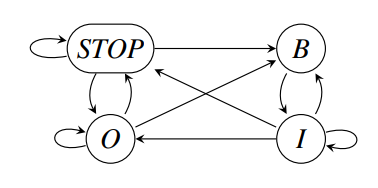
\includegraphics[width=\linewidth]{figure1_state_diagram.png}
	\caption{\label{font-table} State transition diagram used in \citet{ponvert-etal-2011-simple} }
\end{figure}

The cascading aspect of this algorithm can be formulated as follows, using an example from \citet{ponvert-etal-2011-simple} rephrased for clarity over brevity:

\begin{enumerate}
	\item Start with raw tokenized text:
		
	\begin{center}\emph{There is no asbestos in our products now}\end{center}	
	
	\item Apply the model using the Viterbi algorithm:	
	
	\begin{center}\emph{There (is no asbestos) in (our products) now}\end{center}	
	
	\item Replace chunks with pseudowords:	
	
	\begin{center}\emph{There \fbox{is} in \fbox{our} now}\end{center}	
	
	\item Cascade by repeating steps 1--4 on the new sequence while chunks are still found in the sequence:
	
	\begin{center}\emph{(There \fbox{is}) (in \fbox{our}) now}\end{center}
	
	\item Unravel to create a parse tree:	
	
	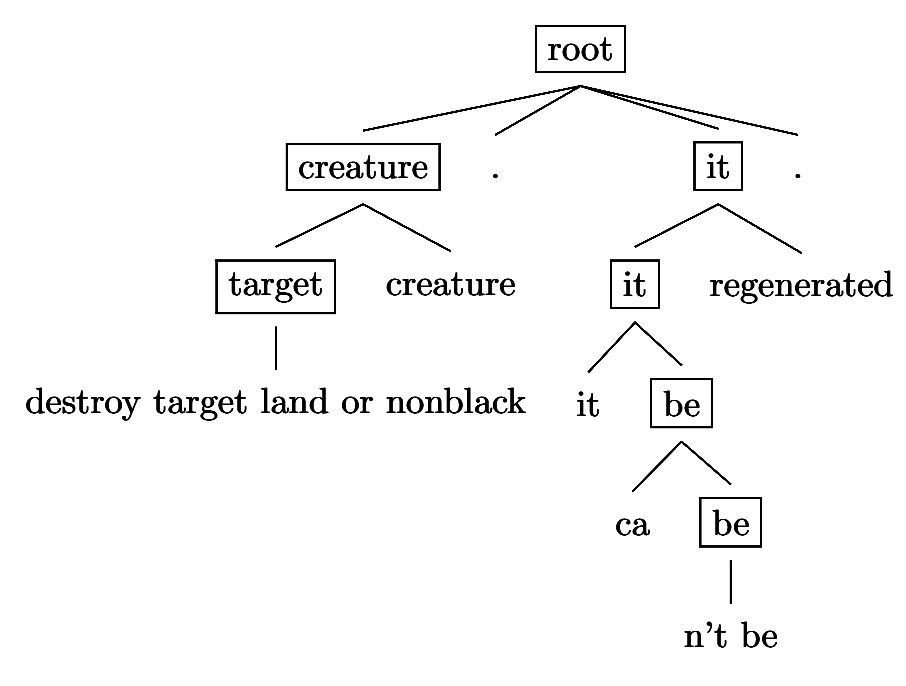
\includegraphics[width=\linewidth]{parse_tree_example.png}
\end{enumerate}

This process can be described as applying the chunking models in layers.
After a given layer is chunked, the chunk is replaced with a pseudoword.
\citet{ponvert-etal-2011-simple} found that using the token in the chunk with the highest corpus frequency was simple, but provided effective results.
Additionally, the chunkers used at each level were initialized with the same parameters, tokens, and smoothing.

\section{Evaluation and Testing}

Like the original paper, we will base our evaluation on identifying multi-word chunks of all constituent types as well as noun phrases (NPs).
We will test our model on the dataset from the Conference in Computational Natural Language Learning (CoNLL-2000) chunking task \footnote{\url{https://www.clips.uantwerpen.be/conll2000/chunking/}} to ensure our model is correctly implemented.
Once we have verified this, we will see what results we get for the TCG datasets.
We will utilize PRLG, as our primary evaluation model and compare it against an HMM model as a benchmark.
This will allow us to validate our results as information is lost due to the independence assumption characteristic of an HMM model.
By comparing it against PRLG we should expect PRLG to perform better as referenced in the original paper.
Model performance is primarily reported on the results from computing language model perplexity.
Furthermore, we may compute precision, recall and F-score for full constituent identification.

We will initially split our dataset into 60\% for training, 20\% for dev and 20\% for testing.
During training we will keep the evaluation sets blind to the model.
We will use the 10-fold cross validation method with bootstrapping to ensure statistical significance.
Finally, we will experiment with a few variations of preprocessing the TCG rules.
For example, we will compare a control model to one that replaces a card’s name with a terminal token \textless this\textgreater, and one that replaces consecutive digits with the token \textless number\textgreater.

\section{Progress}

We began by collecting the data we would need to build our models.
Data was accessed through MTGJSON \footnote{\url{https://mtgjson.com/}}, an open source project that catalogues all current MTG cards.
The extracted data was then formatted for us to better analyze: we chose to use a tuple of the card name and rules text so we can complete the comparison of the control model like we had planned.
The data was also split into the proposed testing, development, and training sections.
Base HMM and PRLG implementation classes were completed, as well as code to execute the Forward, Backward, and Viterbi algorithms.
Our next steps include finishing the development of the Baum-Welch algorithm to find the unknown parameters of the HMM, implement cascading to follow our proposed solution, test and evaluate our work and make possible adjustments, and we also plan on integrating our work onto other available card games like YuGiOh. 

\section{Potential Blocks}

One potential block we may encounter regarding TCG datasets that have fewer cards (like \emph{Yu-Gi-Oh!}) is how we split the dataset.
We may have to use smaller dev and test portions because these games have less data to train on.

Another potential issue that we had anticipated was in evaluating the model on the TCG cards.
The original paper calculated precision, recall, and F-scores based on the performance of the model specifically regarding chunking NPs and other constituent types.
Because the TCG data is unlabeled, to address this issue, we discovered that we can use perplexity as an evaluation metric.
We may also confirm that the rules text that includes a card’s name forms constituents.

We had come across a block where we needed a large dataset to test our model on.
We began by attempting to acquire the English Treebank-3, Chinese Treebank 5.0, and the NEGRA Corpus to have a much larger scale corpus to test on, but we quickly found out that those datasets required either a research license or a large sum of money to use.
Our solution is to use the CoNLLU dataset.

\bibliography{anthology,acl2020}
\bibliographystyle{acl_natbib}

\end{document}
